\section{Code Generation}
Nearing the end, of the compiler, after doing all the contextual analysis, you end up with a decorated syntax tree which has made sure that everything lives up to the programming language that has got defined earlier in this report. Now it’s time for code generation.
Here there can be multiple code generators, as it can follow the visitor pattern to generate the code. This is the point where the designer of the compiler decides what the resulting language of the compiler should be. Whenever it should be C, Assembly, etc. It depends on what we design the programming language for. Sometimes it might be necessary to make some pre-defined code to support the structures and functionality of the programming language.
A good approach might be to create an intermediate language if you want to compile multiple high-level programming languages to a low-level programming language. In that way instead of making many compilers from D => B, E => B, D => C, E => C, you can create one compiler from the high-level language to the intermediate language. If you want to output to multiple low-level languages, you need to add another compiler from the intermediate language to the new low-level language. In that way, instead of making a high-level \* low-level number of compilers, make High-level \+ Low-level number of compilers. It adds abstraction but might also add complexity if either the source language or the destination language has structures that are hard or impossible to implement. Some examples of compilers with intermediate languages are Java and C\#. Java compiles Java Bytecode which is the instruction set of the Java Virtual Machine. C\# compiles to Common Intermediate Language, which is then run on the Common Language Runtime.\\
\\
Taken a look into the code generation. There are 3 code generator visitors in total. The first one being C Code Generator, which is generating C code from the AST visitor. The second one is Arduino C code generator, which has the special features from the Arduino library, for example serial.print and many more. The last one is Java Bytecode generator for Jasmin. As there is a lot of code in these generators, and visitors has been explained in the previous chapter, we will focus on the code generation part from each of these code generator visitors.
The first code snippet is from the C code generator visitor, which are using its start node to include the necessary C headers within the generated code : \\
\begin{figure}[H]
\centering
\frame{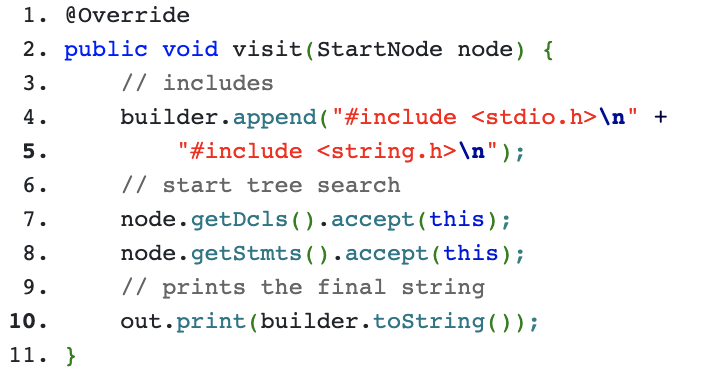
\includegraphics[scale=0.70]{figures/ew/io01.png}}
\label{io01}
\end{figure}
The second case, is where we have the Arduino C code generator.
\begin{figure}[H]
\centering
\frame{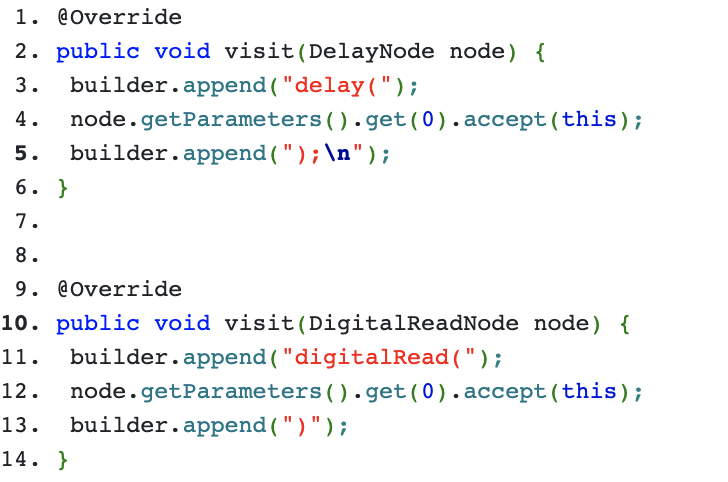
\includegraphics[scale=0.70]{figures/ew/io02.png}}
\label{io02}
\end{figure}
In example on figure \ref{io02}, we got two visitor function, both the delay node and the digital read node. Each of these will append the special Arduino library functions to the code generator, if it read the function id as both within the buildastvisitor. \\
\\
The last visitor is the Jasmin byte code visitor.\\
\begin{figure}[H]
\centering
\frame{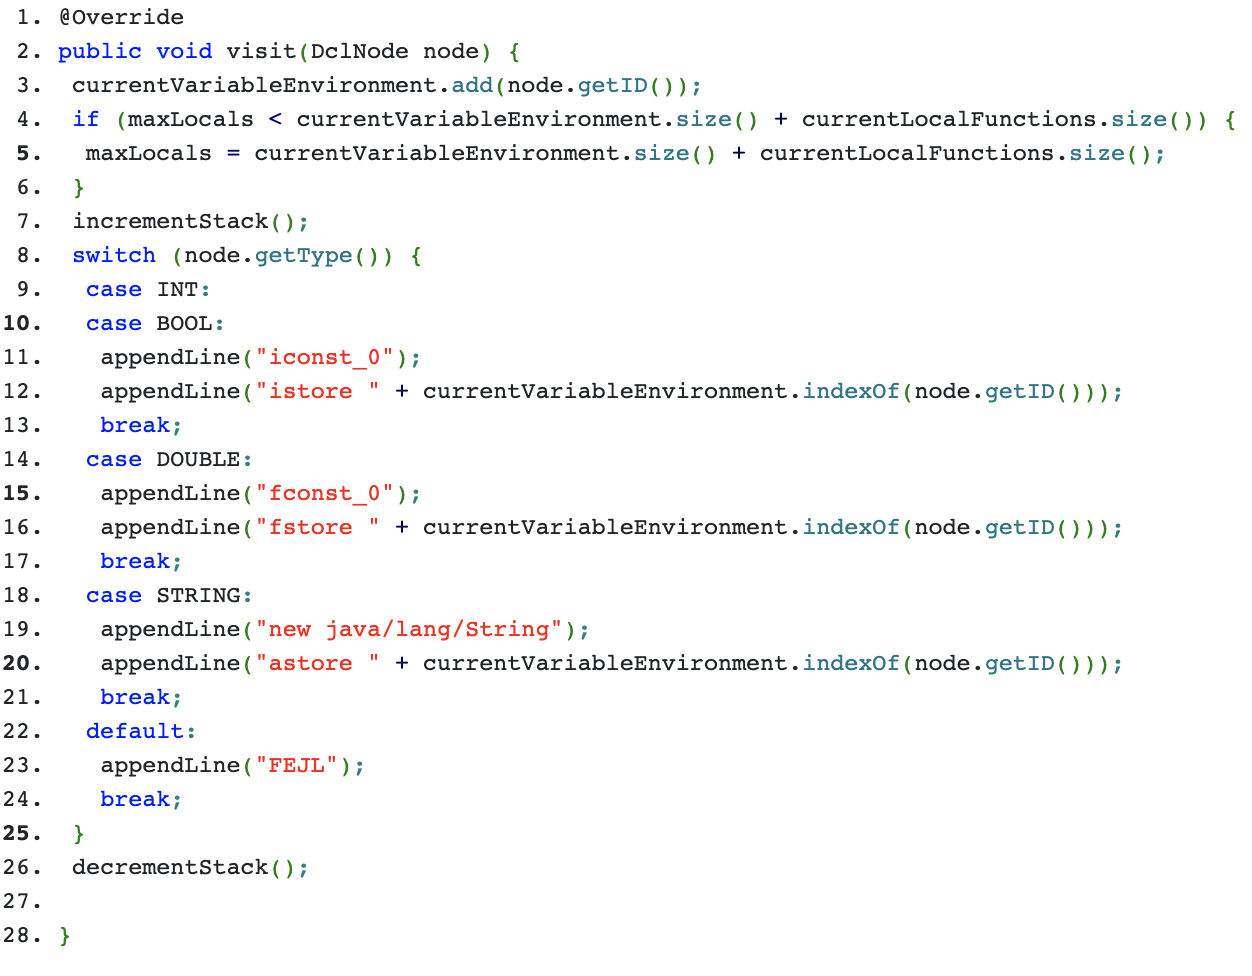
\includegraphics[scale=0.65]{figures/ew/io03.png}}
\label{io03}
\end{figure}
